\RequirePackage{ifthen}
\RequirePackage{xargs}
\RequirePackage{tikz}
\RequirePackage{tkz-tab}
\usetikzlibrary{shadows,decorations.pathmorphing,calc,backgrounds,tikzmark}

\newcommand{\reperevl}[4] %(xmin,ymin,xmax,ymax)
{
	\draw [thin, quadrillage@color](#1,#2) grid (#3,#4);
	\draw [thick, black] (#1,0) -- (#3,0);
	\draw [thick, black] (0,#2) -- (0,#4);
	\draw [ black](0,0) node[below left] {O};
	\draw [thick, ->,>=latex,black] (0,0) -- (1,0) node[midway,below]  {\footnotesize $\vv{\imath}$};
	\draw [thick, ->,>=latex,black] (0,0) -- (0,1) node[midway,left]  {\footnotesize $\vv{\jmath}$};
}

\newcommand{\reperev}[4] %(xmin,ymin,xmax,ymax)
{
	\draw [very thin, color = quadrillage@color!50, step = .5](#1,#2) grid (#3,#4);
	\draw [thin, color = quadrillage@color](#1,#2) grid (#3,#4);
	\draw [thick,color = black] (#1,0) -- (#3,0);
	\draw [thick,color = black] (0,#2) -- (0,#4);
	\draw [color = black](0,0) node[below left] {O};
	\draw [thick, ->,>=latex,color = black] (0,0) -- (1,0) node[midway,below]  {\footnotesize $\vv{\imath}$};
	\draw [thick, ->,>=latex,color = black] (0,0) -- (0,1) node[midway,left]  {\footnotesize $\vv{\jmath}$};
}

\newcommand{\repereal}[4] %(xmin,ymin,xmax,ymax)
{
	\draw [thin, quadrillage@color](#1,#2) grid (#3,#4);
	\draw [->,>=latex, thick] (#1,0) -- (#3,0);
	\draw [->,>=latex, thick] (0,#2) -- (0,#4);
	\draw (0,0) node[below left] {O};
	\draw (1,0) node[below left] {I} node {\tiny $|$};
	\draw (0,1) node[left] {J} node[rotate =90] {\tiny $|$};
}

\newcommand{\reperenb}[6] %(xmin,ymin,xmax,ymax,xlabel,ylabel)
{
	\scriptsize
	\newcount\Ubeg
	\newcount\Uend
	\def\ecart{-.2}

	\draw [thin, quadrillage@color](#1,#2) grid (#3,#4);
	\draw [->,>=latex, thick] (#1,0) -- (#3,0);
	\draw [->,>=latex, thick] (0,#2) -- (0,#4);

	\Ubeg #1\relax
	\advance\Ubeg +1\relax
	\Uend #3\relax
	\advance\Uend -1\relax

	\foreach \x in {\the\Ubeg,...,\the\Uend}
		{
			\draw[thick] (\x,-.05)--(\x,.05);
			\node at (\x+\ecart,\ecart){\x};
		}

	\Ubeg #2\relax
	\advance\Ubeg +1\relax
	\newcount\Uend
	\Uend #4\relax
	\advance\Uend -1\relax

	\foreach \x in {\the\Ubeg,...,\the\Uend}
		{
			\draw[thick] (-.05,\x)--(.05,\x);
			\node at (\ecart,\x+\ecart){\x};
		}
    \draw (#3,0) node[above left]{#5};
    \draw (0,#4) node[rotate = 90, below left]{#6};
}

\newcommand{\reperea}[4] %(xmin,ymin,xmax,ymax)
{
	\draw [very thin, quadrillage@color!50, step = .5](#1,#2) grid (#3,#4);
	\draw [thin, quadrillage@color](#1,#2) grid (#3,#4);
	\draw [->,>=latex, thick] (#1,0) -- (#3,0);
	\draw [->,>=latex, thick] (0,#2) -- (0,#4);
	\draw (0,0) node[below left] {O};
	\draw (1,0) node[below left ] {I} node {\tiny $|$};
	\draw (0,1) node[left] {J} node[rotate =90] {\tiny $|$};
}

\newcommand{\reperecompl}[4] %(xmin,ymin,xmax,ymax)
{
	\draw [thin, quadrillage@color](#1,#2) grid (#3,#4);
	\draw [->,>=latex, thick] (#1,0) -- (#3,0);
	\draw [->,>=latex, thick] (0,#2) -- (0,#4);
	\draw (0,0) node[below left] {$0$};
	\draw (1,0) node[below] {$1$} node {\tiny $|$};
	\draw (0,1) node[left] {$i$} node[rotate =90] {\tiny $|$};
}

\newcommand{\reperecomp}[4] %(xmin,ymin,xmax,ymax)
{
	\draw [very thin, quadrillage@color!50, step = .5](#1,#2) grid (#3,#4);
	\draw [thin, quadrillage@color](#1,#2) grid (#3,#4);
	\draw [->,>=latex, thick] (#1,0) -- (#3,0);
	\draw [->,>=latex, thick] (0,#2) -- (0,#4);
	\draw (0,0) node[below left] {0};
	\draw (1,0) node[below] {1} node {\tiny $|$};
	\draw (0,1) node[left] {$i$} node[rotate =90] {\tiny $|$};
}

\newcommand{\reperec}[6] %(xmin,ymin,xmax,ymax,xlabel,ylabel)
{
	\draw [very thin, quadrillage@color!50, step = .5](#1,#2) grid (#3,#4);
	\draw [thin, quadrillage@color](#1,#2) grid (#3,#4);
	\draw [->,>=latex, thick] (#1,0) -- (#3,0) ;
	\draw (#3,0) node[below left]{\footnotesize #5};
	\draw [->,>=latex, thick] (0,#2) -- (0,#4);
	\draw (0,#4) node[rotate = 90, above left]{\footnotesize #6};
}

\newcommand{\reperecl}[6] %(xmin,ymin,xmax,ymax,xlabel,ylabel)
{

	\draw [thin, quadrillage@color](#1,#2) grid (#3,#4);
	\draw [->,>=latex, thick] (#1,0) -- (#3,0) ;
	\draw (#3,0) node[below left]{\footnotesize #5};
	\draw [->,>=latex, thick] (0,#2) -- (0,#4);
	\draw (0,#4) node[rotate = 90, above left]{\footnotesize #6};
}

\newcommand{\ball}{node [circle,fill=pointbord@color, inner sep=.12em]{}node [circle,fill=point@color, inner sep=.08em]{}}
\newcommand{\point}[3] %(x,y,name)
{
	\draw [thick, pointilles@color, dashed](#1,0) -- (#1,#2) \ball -- (0,#2);
	\ifthenelse{\( \lengthtest{#1 cm > 0 cm } \) \AND \( \lengthtest{#2 cm >0 cm } \)}
	{\draw (#1,#2) node[above right]{#3};}
	{}
	\ifthenelse{\( \lengthtest{#1 cm > 0 cm } \) \AND \( \lengthtest{#2 cm<0 cm} \)}
	{\draw (#1,#2) node[below right]{#3};}
	{}
	\ifthenelse{\( \lengthtest{ #1 cm < 0 cm} \) \AND \( \lengthtest{ #2 cm >0 cm} \)}
	{\draw (#1,#2) node[above left]{#3};}
	{}
	\ifthenelse{\( \lengthtest{ #1 cm < 0 cm} \) \AND \( \lengthtest{ #2 cm <0 cm} \)}
	{\draw (#1,#2) node[below left]{#3};}
	{}
}

\newcommand{\pointx}[3] %(x,y,name)
{
	\draw [thick, pointilles@color, dashed](#1,0) -- (#1,#2) -- (0,#2);
	\ifthenelse{\( \lengthtest{#1 cm > 0 cm } \) \AND \( \lengthtest{#2 cm >0 cm } \)}
	{\draw (#1,#2) node[above right]{#3};}
	{}
	\ifthenelse{\( \lengthtest{#1 cm > 0 cm } \) \AND \( \lengthtest{#2 cm<0 cm} \)}
	{\draw (#1,#2) node[below right]{#3};}
	{}
	\ifthenelse{\( \lengthtest{ #1 cm < 0 cm} \) \AND \( \lengthtest{ #2 cm >0 cm} \)}
	{\draw (#1,#2) node[above left]{#3};}
	{}
	\ifthenelse{\( \lengthtest{ #1 cm < 0 cm} \) \AND \( \lengthtest{ #2 cm <0 cm} \)}
	{\draw (#1,#2) node[below left]{#3};}
	{}
}

\newcommand{\pointc}[5] %(x,y,label1,label2,name)
{
	\draw [thick, pointilles@color, dashed](#1,0) -- (#1,#2)\ball -- (0,#2);
	\ifthenelse{\( \lengthtest{#1 cm > 0cm}\)\AND\( \lengthtest{#2 cm>0 cm }\)}
	{\draw (#1,#2) node[above right]{#5};
		\draw (0,#2) node[left]{#4};
		\draw (#1,0) node[below]{#3};
	}
	{}
	\ifthenelse{\(\lengthtest{#1 cm> 0 cm }\)\AND\( \lengthtest{ #2 cm<0 cm}\)}
	{\draw (#1,#2) node[below right]{#5};
		\draw (0,#2) node[left]{#4};
		\draw (#1,0) node[above]{#3};}
	{}
	\ifthenelse{\(\lengthtest{#1cm < 0cm}\)\AND\(\lengthtest{#2cm>0cm}\)}
	{\draw (#1,#2) node[above left]{#5};
		\draw (0,#2) node[right]{#4};
		\draw (#1,0) node[below]{#3};}
	{}
	\ifthenelse{\(\lengthtest{#1cm <0cm}\)\AND\(\lengthtest{#2cm<0cm}\)}
	{\draw (#1,#2) node[below left]{#5};
		\draw (0,#2) node[right]{#4};
		\draw (#1,0) node[above]{#3};}
	{}
}

\newcommand{\pointcx}[5] %(x,y,label1,label2,name)
{
	\draw [thick, pointilles@color, dashed](#1,0) -- (#1,#2) -- (0,#2);

	\ifthenelse{\( \lengthtest{#1 cm > 0cm}\)\AND\( \lengthtest{#2 cm>0 cm }\)}
	{\draw (#1,#2) node[above right]{#5};
		\draw (0,#2) node[left]{#4};
		\draw (#1,0) node[below]{#3};
	}
	{}
	\ifthenelse{\(\lengthtest{#1 cm> 0 cm }\)\AND\( \lengthtest{ #2 cm<0 cm}\)}
	{\draw (#1,#2) node[below right]{#5};
		\draw (0,#2) node[left]{#4};
		\draw (#1,0) node[above]{#3};}
	{}
	\ifthenelse{\(\lengthtest{#1cm < 0cm}\)\AND\(\lengthtest{#2cm>0cm}\)}
	{\draw (#1,#2) node[above left]{#5};
		\draw (0,#2) node[right]{#4};
		\draw (#1,0) node[below]{#3};}
	{}
	\ifthenelse{\(\lengthtest{#1cm <0cm}\)\AND\(\lengthtest{#2cm<0cm}\)}
	{\draw (#1,#2) node[below left]{#5};
		\draw (0,#2) node[right]{#4};
		\draw (#1,0) node[above]{#3};}
	{}
}

\newcommand{\secteur}[3]   % {x,y,angledepart,anglefin}
{
	\draw (#1)  ++(#2:.2) arc (#2:#3:.2);
}


\newcommand{\petitscarreaux}[2]
{
	\begin{tikzpicture}
		\draw[fill = white](0,0) rectangle (#1,#2);
		\draw[thin,UGLiBlue!20,step=.5,ystep=.5](0,0) grid (#1,#2);
		\draw[UGLiBlue!30,step=1,ystep=1](0,0) grid (#1,#2);
	\end{tikzpicture}
}
\newcommand{\carreauxseyes}[2]
{
	\begin{tikzpicture}
		\draw[fill = white](0,0) rectangle (#1,#2);
		\draw[quadrillage@color!20,thin,ystep=.2,xstep=.8] (0,0) grid (#1,#2);
		\draw[quadrillage@color!70,step=.8,ystep=.8](0,0) grid (#1,#2);
	\end{tikzpicture}
}


\def\abun{ab1}
\def\abeux{ab2}
\def\abtrois{ab3}
\def\abquatre{ab4}
\def\abcinq{ab5}
\def\absix{ab6}

\def\alun{al1}
\def\aleux{al2}
\def\altrois{al3}
\def\alquatre{al4}
\def\alcinq{al5}
\def\alsix{al6}

\newcommand{\arbreproba}%arbre type bac tes {A}{B}{C}
{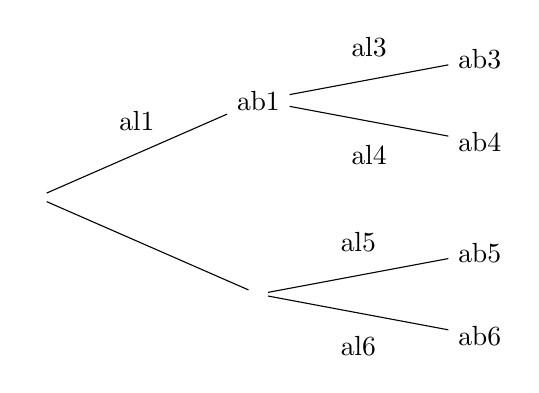
\begin{tikzpicture}[grow = right,level distance=8em,level 1/.style={sibling distance=7em},
			level 2/.style={sibling distance=3em}]
		\node {}
		child {
				node {\abdeux}
				child {
						node 	{\absix} edge from parent node[below=.5em]
							{\alsix}} child {node {\abcinq}edge from parent node[above=.5em]
							{\alcinq}}edge from parent node[below=.5em] {\aldeux}}
		child {node {\abun} child {node {\abquatre} edge from parent node[below=.5em] {\alquatre}} child {node {\abtrois}edge from parent node[above=.5em]
							{\altrois}}edge from parent node[above=.5em] {\alun}};
	\end{tikzpicture}}
